\begin{titlepage}
    \begin{center}
        \thispagestyle{empty}
        \begin{figure}
            \centering
            
\includegraphics[scale=1.15]{F:/Root Files/Academic/masters/_desenvolvimento/_regular/_dissertacao/fase final/_estrutura/_texto/tex/figures/brasao-rep-br.png}
        \end{figure}
        \vspace*{0.1cm}
        \textbf{\large Universidade Federal do Espírito Santo}\\
        \large Centro de Artes\\
        \large Programa de Pós-Graduação em Arquitetura e Urbanismo\\
        \vspace*{3cm}
        \textbf{\large Anderson Azevedo Fraga}\\
        \vspace*{4cm}
        \textbf{Potencial de Adoção do Conceito Zero Energy para Edifícios Comerciais em Vitória-ES}\\
        \vfill % preenche em branco o espaço até o final da página
        Vitória\\
        2020\pagebreak

        \begin{figure}
            \thispagestyle{empty} % limpa cabeçalho, rodapé e número de página
            \centering
            
\includegraphics[scale=1.15]{F:/Root Files/Academic/masters/_desenvolvimento/_regular/_dissertacao/fase final/_estrutura/_texto/tex/figures/brasao-rep-br.png}
        \end{figure}
        \vspace*{0.1cm}
        \textbf{\large Universidade Federal do Espírito Santo}\\
        \large Centro de Artes\\
        \large Programa de Pós-Graduação em Arquitetura e Urbanismo\\
        \vspace*{3cm}
        \textbf{\large Anderson Azevedo Fraga}\\
        \vspace*{4cm}
        \textbf{Potencial de Adoção do Conceito Zero Energy para Edifícios Comerciais em Vitória-ES}\\
        \vspace*{1cm}
            \hfill\begin{minipage}{0.5\linewidth}
            \normalsize Dissertação presentada ao Programa
            de Pós-Graduação em Arquitetura e
            Urbanismo da Universidade Federal do
            Espírito Santo, como requisito para
            obtenção do grau de Mestre em
            Arquitetura e Urbanismo, na área de
            concentração de Arquitetura e
            Urbanismo.\\
            Orientadora: Prof.ª Dr.ª Cristina Engel de
            Alvarez
            \end{minipage}            
        \vfill % preenche em branco o espaço até o final da página
        Vitória\\
        2020\pagebreak

        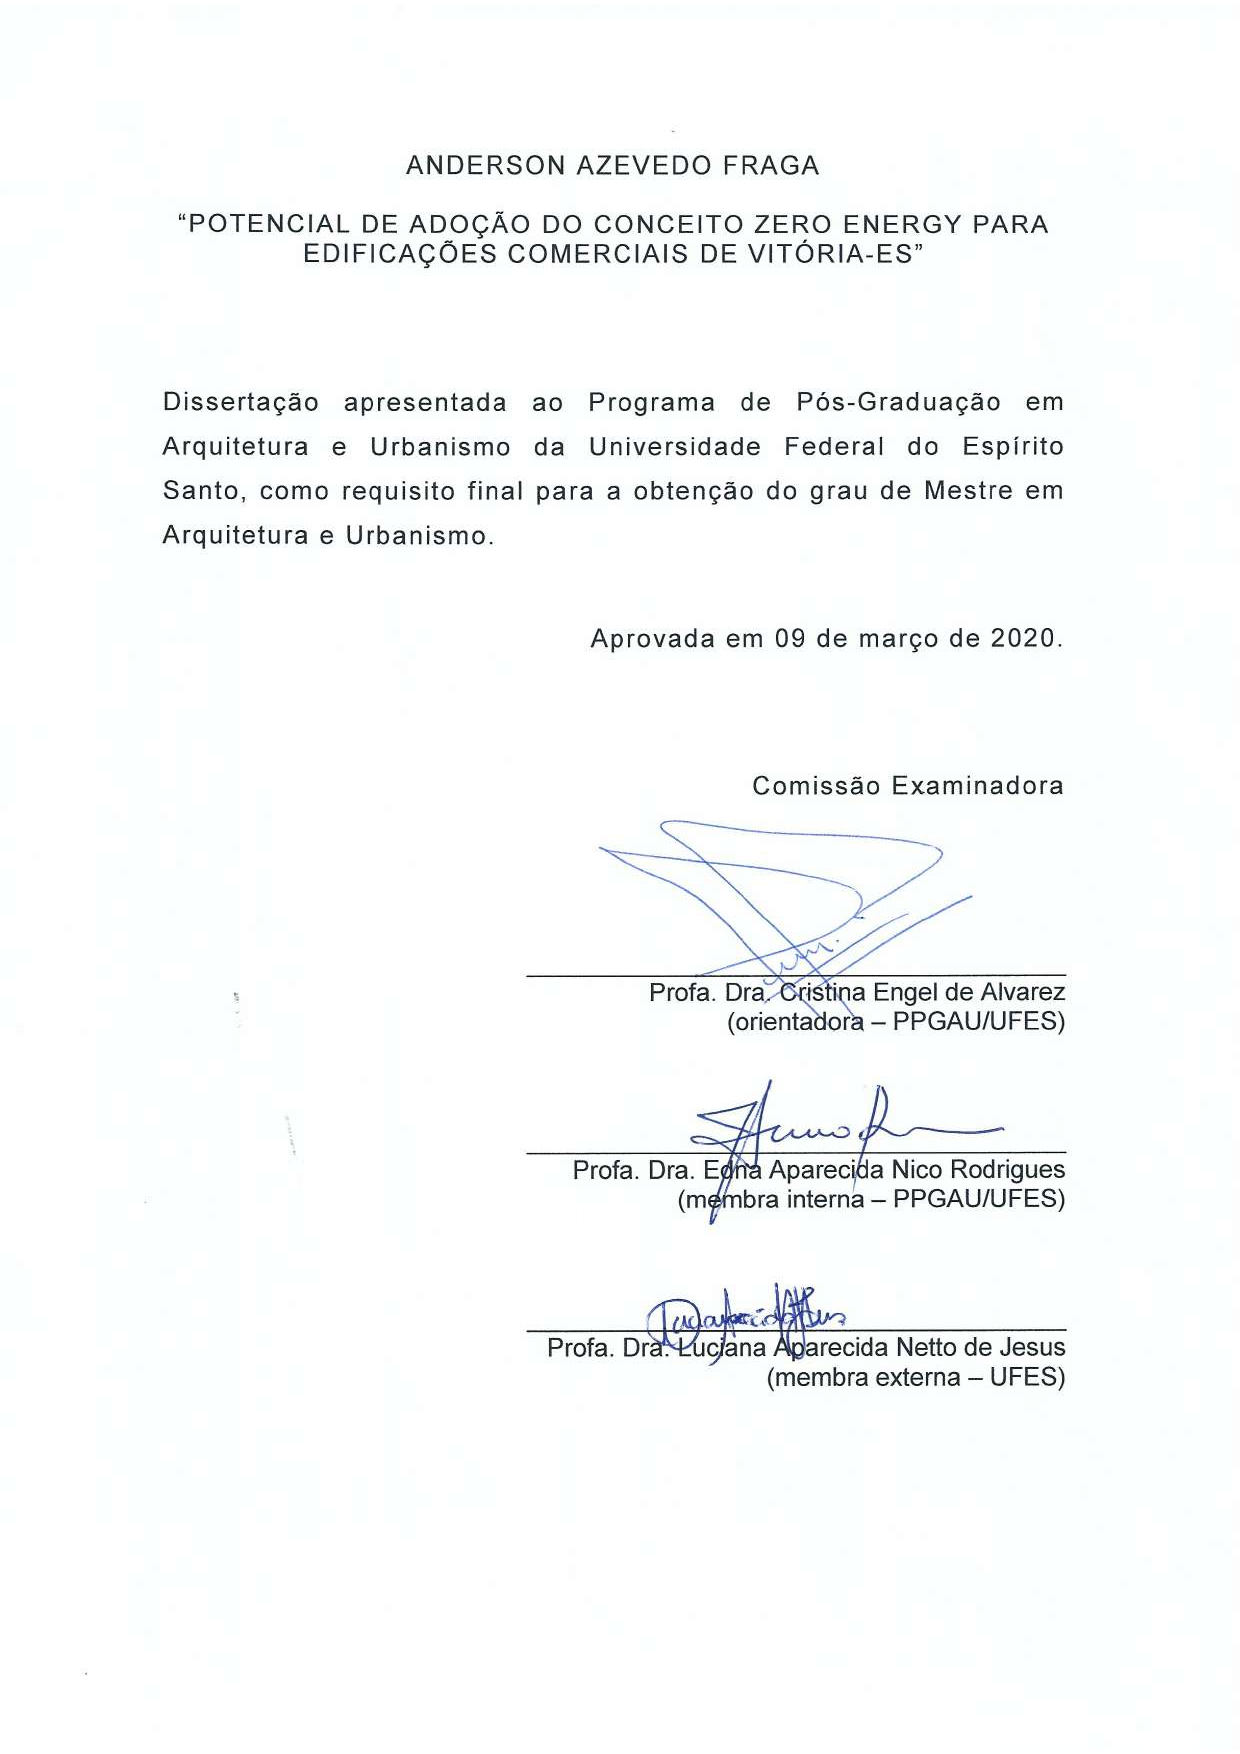
\includepdf[pages=-]{F:/Root Files/Academic/masters/_desenvolvimento/_regular/_dissertacao/fase final/_estrutura/_texto/folha.pdf}\pagebreak

        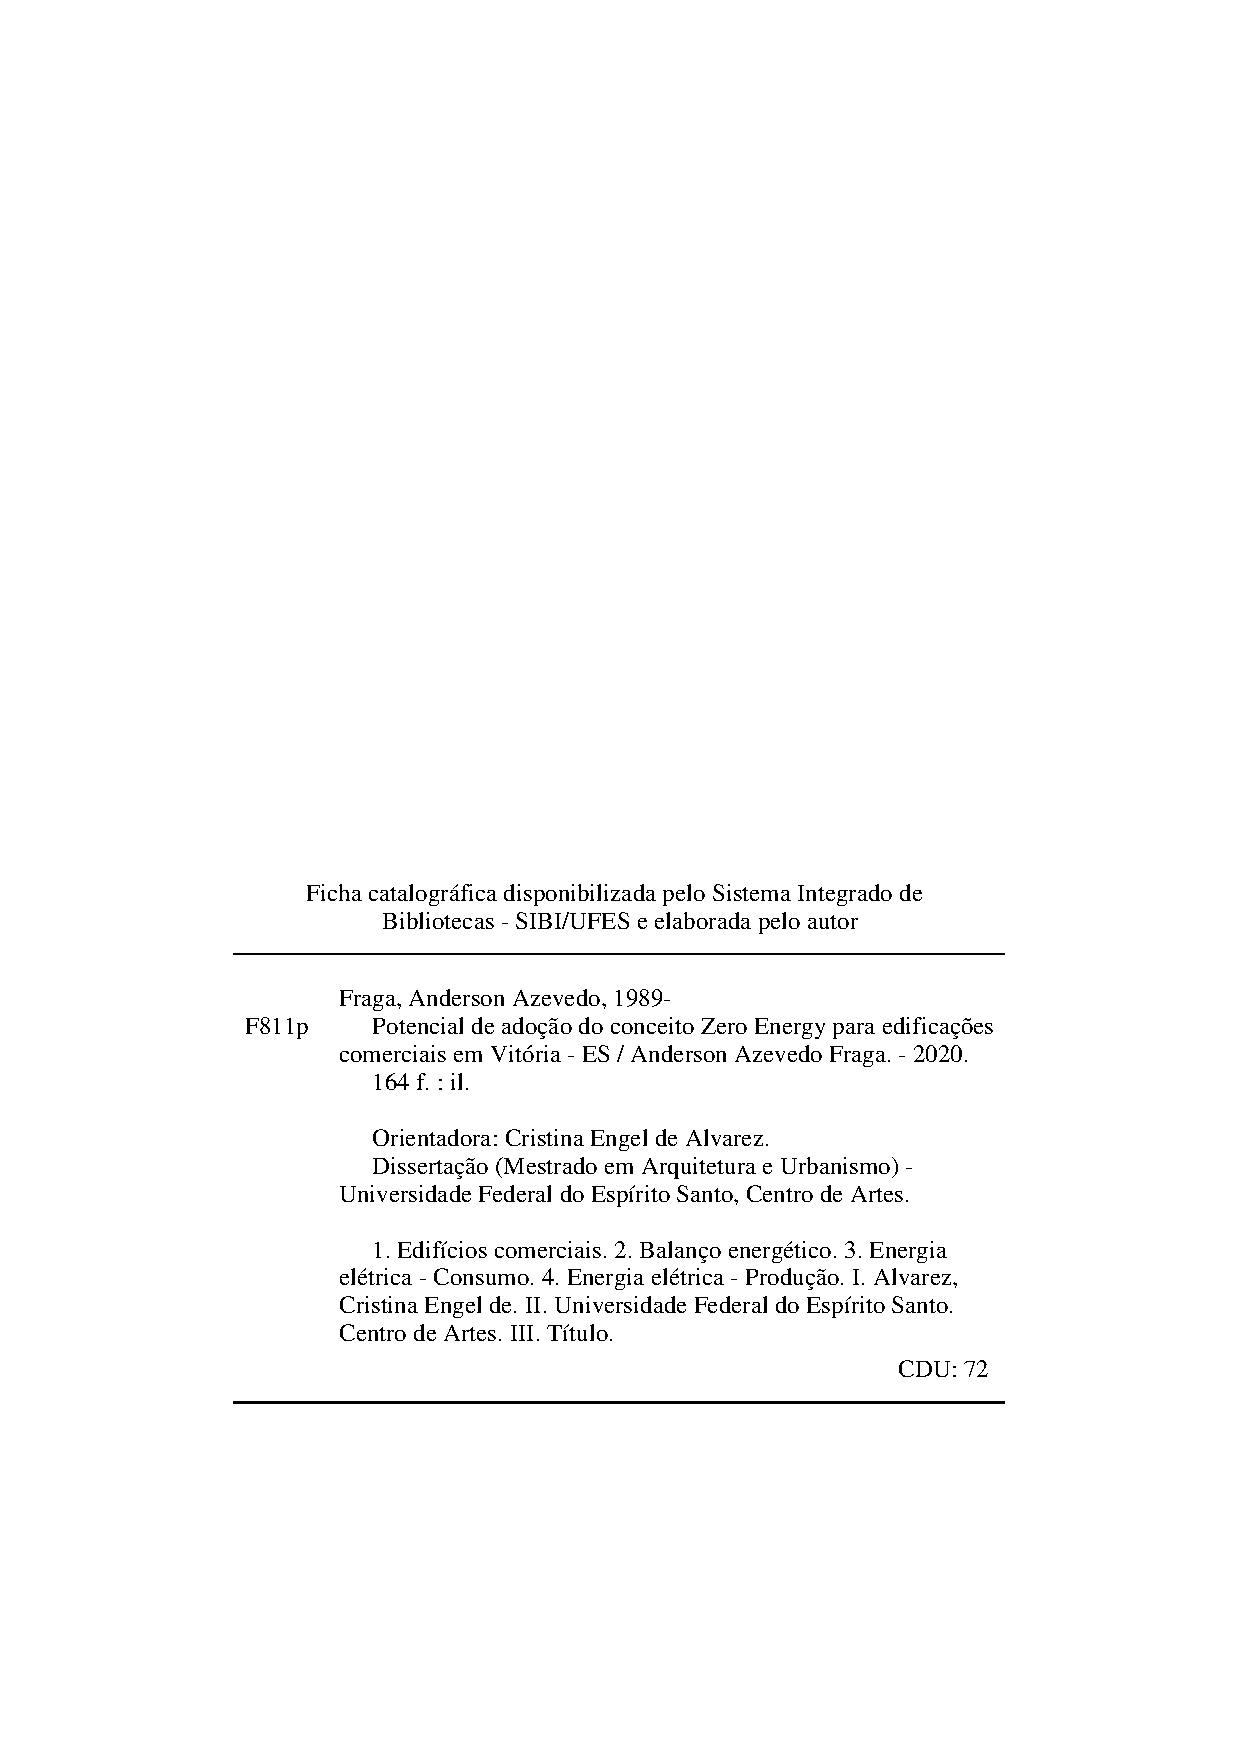
\includepdf[pages=-]{F:/Root Files/Academic/masters/_desenvolvimento/_regular/_dissertacao/fase final/_estrutura/_texto/ficha.pdf}\pagebreak
        
        \thispagestyle{empty}
        \vspace*{\fill}
        \begin{flushright}
            \textit{\itshape A inteligência é o farol que nos guia, mas é a vontade que nos faz caminhar.}\newline
            \textbf{Érico Veríssimo}
        \end{flushright}
        
    \end{center}
\end{titlepage}